\section{Analysis of Number of Bases}

We conduct a hyperparameter sweep over the number of bases $\mathbf{B}$ from 1-20 per scene for the SoM baseline to analyze its behaviour as more distinct transforms are used to model the scene.
We track training/test PSNR as $B$ increases and examine how Gaussian basis blending weights are distributed across bases, on the benchmarks DyCheck~\cite{gao2022dynamic} dataset and NVIDIA dataset~\cite{yoon2020novel}~\ref{fig:sweep-avg}. 
Fig.~\ref{fig:basis-psnr} shows test PSNR saturates as early as 3 bases while training PSNR keeps rising, indicating overfitting rather than better motion modeling.

% Was an inline wrapfigure in sec/4_method.tex (workshop version); caption = its commented-out caption.
\begin{figure}[t]
  \centering
  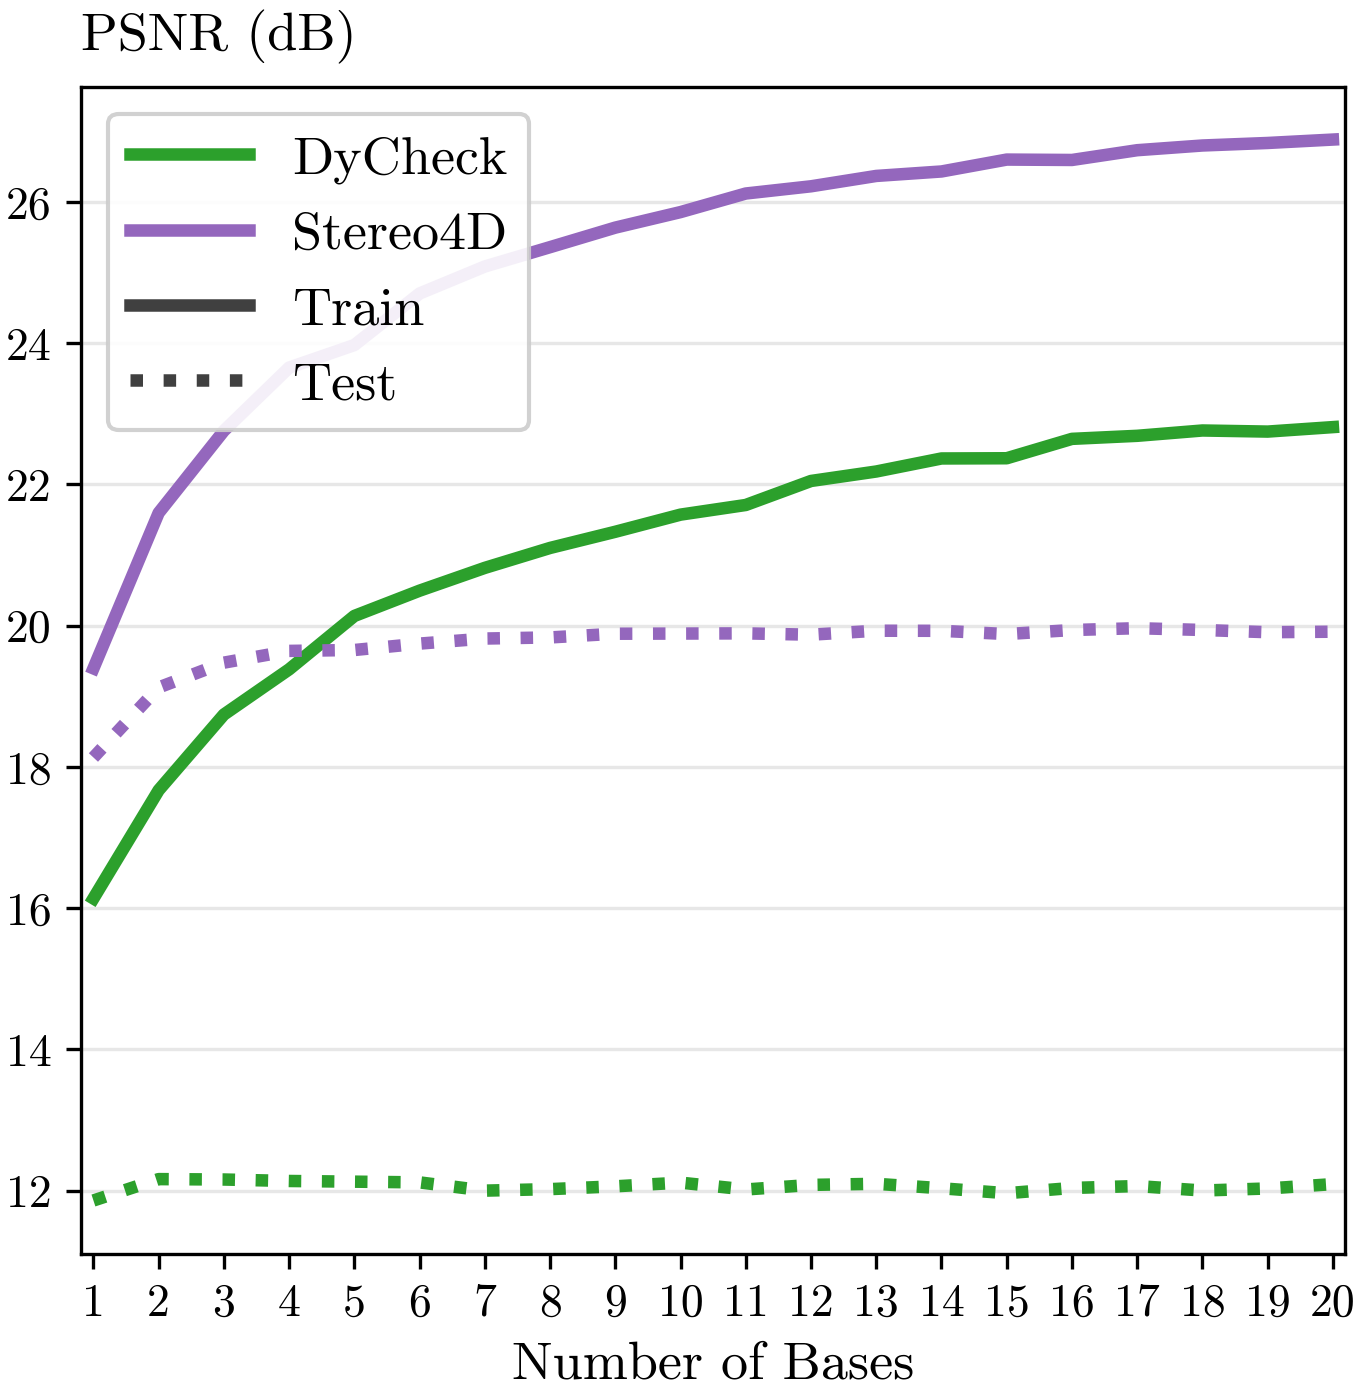
\includegraphics[width=0.75\linewidth]{img/combined-sweep.png}
  \caption{Training PSNR rises with more bases, while test PSNR quickly saturates. \lulu{Replace with NVIDIA instead of stereo}}
  \label{fig:basis-psnr}
\end{figure}


% % Was a commented-out wrapfigure in sec/4_method.tex (workshop version); caption = its commented-out caption.
% Label renamed from fig:basis-utilization, which fig/synthetic_weights.tex uses.
\begin{figure}[t]
  \centering
  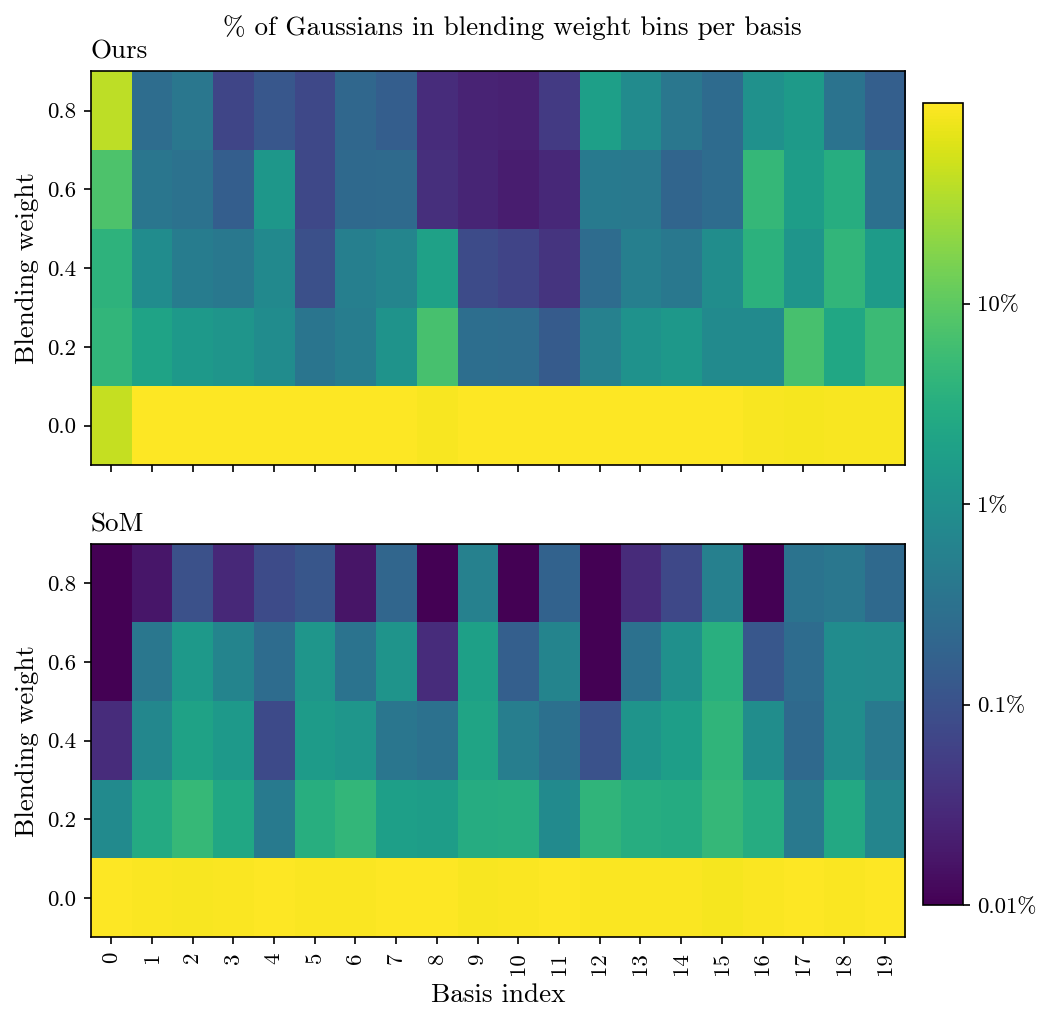
\includegraphics[width=\linewidth]{img/heatmap.png}
  \caption{Average Gaussian basis blending weights across bases.}
  \label{fig:basis-utilization-heatmap}
\end{figure}


In addition to standard benchmarks, we construct a synthetic pinwheel scene with two motion modes: a dominant rotation about the center and a localized translation of the blade tips, affecting roughly $20\%$ of the tracks. The inset compares the average blending weight assigned to each basis after fitting SoM. With 20 bases, SoM assigns substantial, nearly uniform weight across many bases, failing to reflect the underlying two-mode structure. The additional capacity is instead used to minimize the training-view photometric loss, producing noisy, overfit trajectories. This suggests that increasing the number of bases weakens the regularization provided by the compact 3--5 basis model. As a preview of our approach, the weighting profile shown in the inset instead concentrates motion in a few bases, while reserving other bases for smaller residual motions. We formalize this idea through the incremental optimization scheme introduced in the next section.

